\chapter{Results}
\label{chap:results}
In this chapter I present visual results for the roads that are imported into the snow simulator, and some performance analysis of the road generator. 

\section{Test bench hardware}
All tests and renderings were performned on a desktop computer with the specifications given in table \ref{tab:testspecs}. 
\begin{table}[ht]
\centering
\begin{tabular}{lll}
\hline
\tbf {Component} & \tbf {Specifications} & \tbf {Remarks}\\
\hline
CPU      & Intel Core(tm)2 Quad Q9550 2.83GHz & \\
L1 Cache & 64KB                               & 32KB data, 32KB instruction\\
L2 Cache & 12MB                               & Unified; two cores share 6MB\\
Memory   & 4GB & \\
GPU 1    & NVIDIA Quadro FX 5800              & \\
GPU 2    & NVIDIA Tesla C1060                 & GPU used for the GPU computing tasks\\
\hline
\end{tabular}
\caption{Hardware specifications for test bench}
\label{tab:testspecs}
\end{table}
The Tesla C1060 device was used for all GPU computing tasks.

\section{Visual results}
In this section, we will look at visual results for the generated roads; both as an overlay to the heightmap, and some of the generated roads imported into the snow simulator. All roads have a starting point at position $(0,0)$, i.e. lower left corner of the heightmap, and a end position at the upper right corner.

First, we look at the road trajectories that are generated for different height maps. These are shown in figure \ref{fig:road_trajectory}. Figure \ref{fig:trajectory_mountains} shows an automatically generated terrain (a fractal terrain) representing a mountainous terrain, and a valley. Figures \ref{fig:trajectory_helens_before} and \ref{fig:trajectory_helens_after} is heightmaps representing Mt. St. Helens before and after the erruption; this is terrains converted from actual digital elevation maps (see \cite{helens_dem} for the source DEMs). We see that generally, the trajectories seem to follow the terrain contour lines, as this minimizes the slope cost of the path, which is what was expected. 

\begin{figure}[ht]
\centering
\subfloat[Autogenerated mountainous terrain]{\label{fig:trajectory_mountains}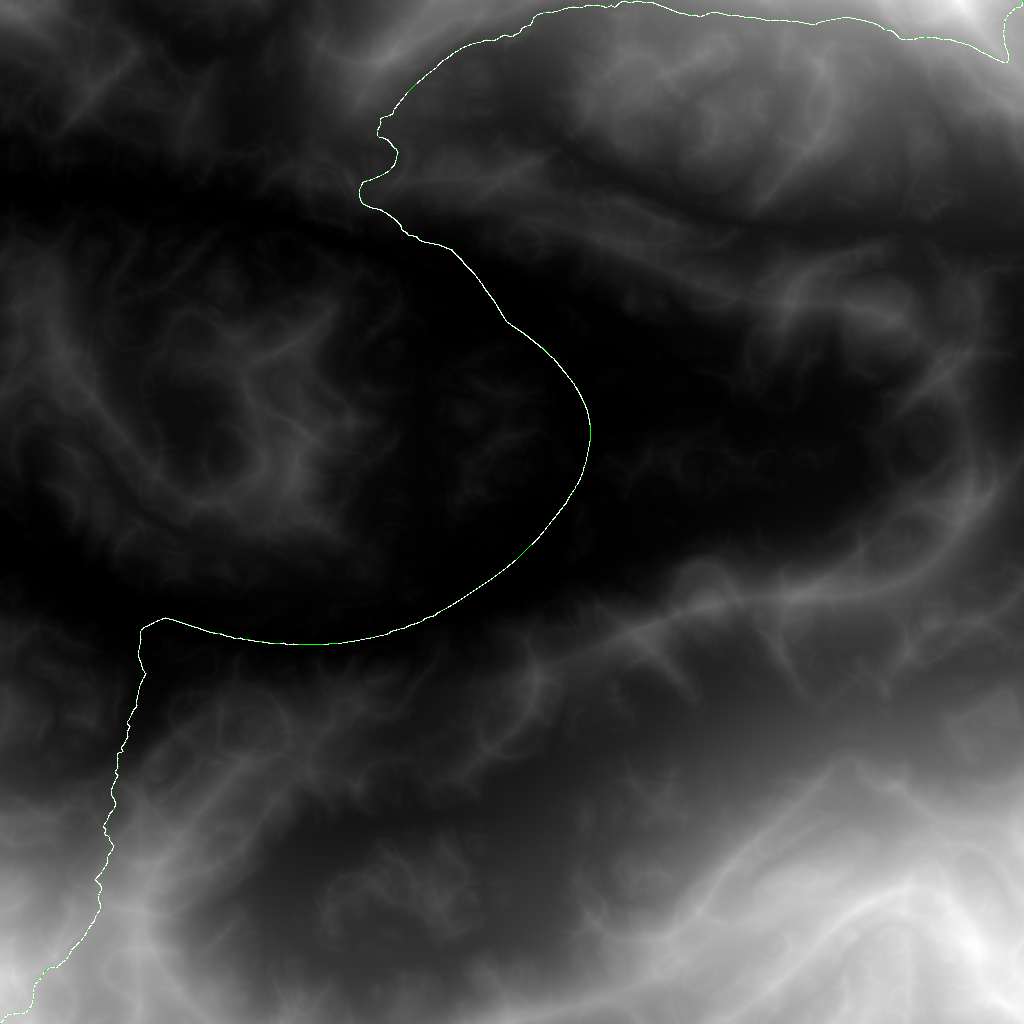
\includegraphics[width=1\textwidth]{figure/trajectory_mountains}}\\
\subfloat[Mount St. Helens (before erruption)] {\label{fig:trajectory_helens_before}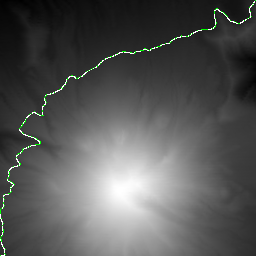
\includegraphics[width=0.485\textwidth]{figure/trajectory_helens_before}}\quad
\subfloat[Mount St. Helens (after erruption)]{\label{fig:trajectory_helens_after}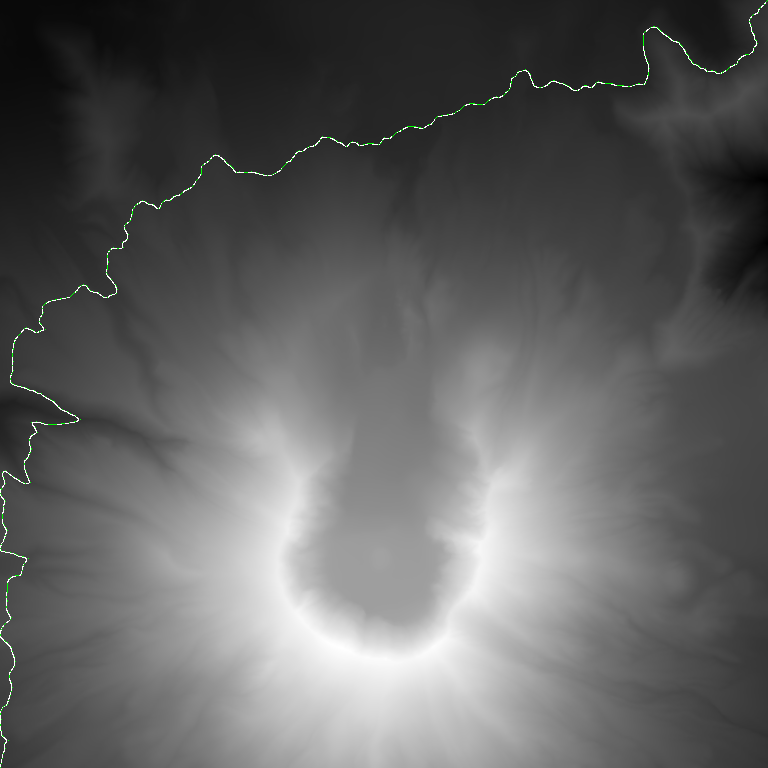
\includegraphics[width=0.485\textwidth]{figure/trajectory_helens_after}}
\caption{Procedurally generated road trajectories for different heightmaps}
\label{fig:road_trajectory}
\end{figure}

\begin{figure}[ht]
\centering
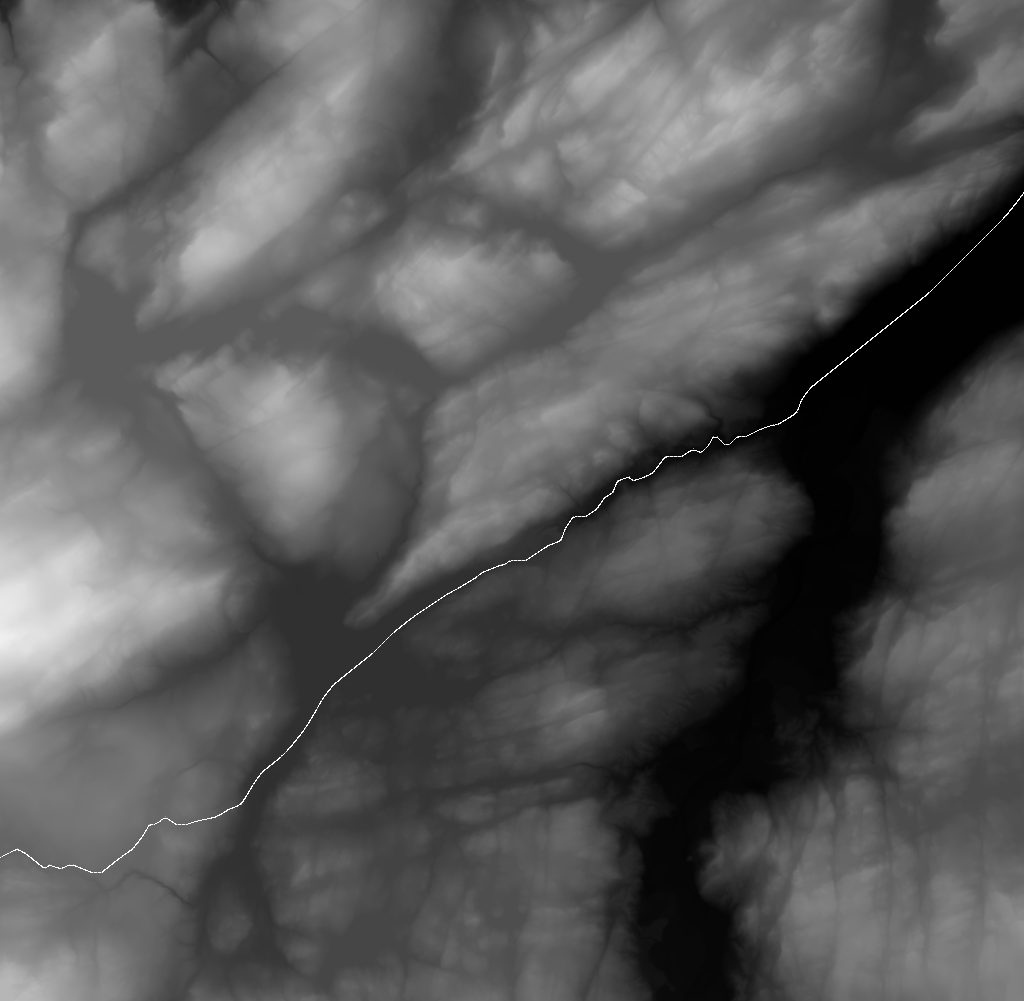
\includegraphics[width=\textwidth]{figure/trajectory_trondheim}
\caption{Procedurally generated road trajectory for Trondheim}
\label{fig:trajectory_trondheim}
\end{figure}

After loading the model into the snow simulator and adjusting the terrain, we can see the roads as it curves through the terrain. Figure \ref{fig:road_in_terrain_nosnow} shows the road and the terrain without snow cover. We clearly see the effects of the terrain adjustments in the bottom two screenshots, i.e. figures \ref{fig:road_in_terrain_nosnow_2} and \ref{fig:road_in_terrain_nosnow_3}. Note that snow rendering was disabled on the overview image (figure \ref{fig:road_in_terrain_nosnow_1}) in order to improve visibility of the road. 

\begin{figure}[ht]
\centering
\subfloat[Terrain overview]{\label{fig:road_in_terrain_nosnow_1}\includegraphics[width=\textwidth]{figure/screenshots/road_nosnow_1_resampled}}\\
\subfloat[Detailed view of road]{\includegraphics[width=0.485\textwidth]{figure/screenshots/road_nosnow_2_resampled}}\quad
\subfloat[Significant terrain adjustments]{\includegraphics[width=0.485\textwidth]{figure/screenshots/road_nosnow_3_resampled}}
\caption{Road and terrain before snowcover}
\label{fig:road_in_terrain_nosnow}
\end{figure}

After some snow has fallen, as in figure \ref{fig:road_in_terrain_nosnow}, the terrain has been more or less covered in snow except for some shadowed areas. The snow height is continously "smoothed", so that snow that falls in areas with a steep gradient in the terrain, is moved downwards along the gradient, simulating sliding snow (think of it as a mini avalanche). We clearly see this effect on the road in figures \ref{fig:road_in_terrain_nosnow_2} and \ref{fig:road_in_terrain_nosnow_3}.

\begin{figure}[ht]
\centering
\subfloat[Snow covered terrain overview]{\label{fig:road_in_terrain_nosnow_1}\includegraphics[width=\textwidth]{figure/screenshots/road_snow_1_resampled}}\\
\subfloat[Snow from higher up covering road]{\label{fig:road_in_terrain_nosnow_2}\includegraphics[width=0.485\textwidth]{figure/screenshots/road_snow_2_resampled}}\quad
\subfloat[Another case of snow sliding down on the road]{\label{fig:road_in_terrain_nosnow_3}\includegraphics[width=0.485\textwidth]{figure/screenshots/road_snow_3_resampled}}
\caption{Road and terrain with snowcover}
\label{fig:road_in_terrain_snow}
\end{figure}

\section{Performance of road generator}
In this section, I present results from performance testing of the road generator. 

\subsection{Testing parameters}
Four different height maps have been tested: digital elevation data from Mt. St. Helens before and after the erruption (from \cite{helens_dem}), a random fractal terrain representing a valley surrounded by mountains, and Trondheim. These maps range from very small to very large, with different resolutions. Table \ref{tab:testmaps} gives an overview of these maps.

\begin{table}[ht]
\centering
\begin{tabular}{lll}
\hline
\tbf{Map} & \tbf{Dimensions} & \tbf{Resolution (m)}\\
\hline
Mt. St. Helens before erruption & $256\times 256$ & $30$\\ 
Mt. St. Helens after erruption  & $768\times 768$ & $10$\\
Random fractal terrain & $1024\times 1024$ & $10$\\
Trondheim & $4096\times 4096$ & $20$\\
\hline
\end{tabular}
\caption{Height maps used for performance testing}
\label{tab:testmaps}
\end{table}

The weights for road length, slope and curvature is set to 1, 100 and 100, respectively. A threshold of maximum curvature was set to 0.03, which is roughly the curvature of a circle with a radius of 33 meters. Paths with an estimated curvature of more than 0.03 is not considered, because these would give unrealistically sharp turns. A neighborhood of $k=5$ is used for all test cases.  This gives 30 neighbors per node, except for the edge nodes which have less.

\subsection{Performance of Dijkstra vs A*}
The main difference between Dijkstra's algorithm and the A* algorithm is that A* takes an estimated guess of the distance to the goal, and uses this, together with the cost to reach the next node from the start, in deciding which node to expand next. With a good heuristic, A* may expand far fewer nodes than Dijkstra's algorithm, typically resulting in a lower search time. In this section I present results where the performance using Dijkstra's algorithm, and the A* algorithm with the heuristic in equation \ref{eq:astar_heuristic} in section \ref{sec:impl_astar}.

\subsection{Effect of grid coarsening}
In this section I present performance results for different densities of grid points. The time used to generate the shortest path and also the optimality of the path, compared to using a density of 1, i.e. where every height point is considered a node in the search graph. The results are presented in table \ref{tab:effect_of_density}. 

\begin{table}[ht]
\centering
\begin{tabular}{ccccc}
\hline
\tbf{Density} & \tbf{Runningtime} & \tbf{Speedup} & \tbf{Road cost} & \tbf{Difference}\\
              &                   &               &                 & \tbf{from "optimal"}\\
\hline
\multicolumn{5}{c}{Mt. St. Helens (before erruption)}\\
\hline
\input{data/helens_before}
\hline
\multicolumn{5}{c}{Mt. St. Helens (after erruption)}\\
\hline
\input{data/helens_after}
\hline
\multicolumn{5}{c}{Mountains}\\
\hline
\input{data/mountains}
\hline
\multicolumn{5}{c}{Trondheim}\\
\hline
\input{data/trondheim}
\hline
\end{tabular}
\caption{Effect of density of grid}
\label{tab:effect_of_density}
\end{table}

We see here that even though a density of one is optimal with regards to cost, which is not surprising because this gives the highest resolution in finding a path, 

